\documentclass[12pt,a4paper]{report}

\usepackage[margin=1in]{geometry}
\usepackage[T1]{fontenc}
\usepackage[utf8]{inputenc}
\usepackage{lmodern}
\usepackage{graphicx}
\usepackage{booktabs}
\usepackage{tabularx}
\usepackage{array}
\usepackage{enumitem}
\usepackage{xcolor}
\usepackage{listings}
\usepackage{tikz}
\usetikzlibrary{positioning,arrows.meta}
\usepackage{fancyhdr}
\usepackage[hidelinks]{hyperref}

\definecolor{ink}{HTML}{172B35}
\definecolor{teal}{HTML}{347C78}
\definecolor{lightgray}{HTML}{F3F4F4}
\hypersetup{
  pdftitle={SCREEN / SENSE: Movie Ratings and Review Sentiment Analysis},
  pdfauthor={Lavanya, Anuj Rawat, Simran Singh, Mahi Tandon}
}

\pagestyle{fancy}
\fancyhf{}
\fancyhead[L]{\small SCREEN / SENSE}
\fancyhead[R]{\small R Programming Project}
\fancyfoot[C]{\thepage}
\setlength{\headheight}{15pt}
\setlist[itemize]{leftmargin=1.5em,itemsep=3pt,topsep=4pt}
\setlist[enumerate]{leftmargin=1.8em,itemsep=3pt,topsep=4pt}
\setlength{\parskip}{5pt}
\setlength{\parindent}{0pt}

\lstset{
  basicstyle=\ttfamily\small,
  backgroundcolor=\color{lightgray},
  frame=single,
  rulecolor=\color{teal},
  breaklines=true,
  columns=fullflexible,
  keepspaces=true,
  showstringspaces=false
}

\begin{document}

% Cover page: names, IDs, faculty, course code, and semester may be edited
% to match the final submission details.
\begin{titlepage}
  \centering
  \vspace*{1.1cm}
  {\Large\bfseries MANAV RACHNA INTERNATIONAL INSTITUTE OF RESEARCH AND STUDIES\par}
  \vspace{0.25cm}
  {\large Department of Computer Science and Engineering\par}
  \vspace{1.6cm}
  {\color{teal}\rule{0.85\textwidth}{1.2pt}\par}
  \vspace{0.5cm}
  {\Huge\bfseries SCREEN / SENSE\par}
  \vspace{0.25cm}
  {\Large Movie Ratings and Audience Review Sentiment Analysis\par}
  \vspace{0.5cm}
  {\color{teal}\rule{0.85\textwidth}{1.2pt}\par}
  \vspace{1.0cm}
  {\large PROJECT-BASED LEARNING REPORT\par}
  \vspace{1.0cm}
  \begin{minipage}{0.78\textwidth}
    \centering
    \textbf{Submitted by}\par\vspace{0.3cm}
    DEEPESH KUMAR SINGH (1/24/SET/BCS/385)\par
    MAYANK CHANDRA (1/24/SET/BCS/390)
   
  \end{minipage}
  \vspace{0.9cm}

  \begin{tabular}{rl}
    \textbf{Subject:} & Programming Using R / Project-Based Learning \\
    \textbf{Academic Year:} & 2026--2027, 5th Semester \\
    \textbf{Submitted to:} & Dr. TANVI CHAWLA \\
    \textbf{Department:} & Computer Science and Engineering
  \end{tabular}
  \vfill
\end{titlepage}

\pagenumbering{roman}
\tableofcontents
\clearpage
\pagenumbering{arabic}

\chapter{Abstract}
SCREEN / SENSE is an interactive R Shiny application for exploring movie ratings, genres, and audience review sentiment. It uses a reproducible sample of 200 films and 6,000 sampled audience reviews. Movie metadata and reviews are stored in CSV files and a local SQLite database. The application lets a user search for a title, inspect its rating and sampled reviews, and compare rating and sentiment patterns across genres and release years. R functions, data frames, conditional logic, data transformation, visualization, and database operations are combined in one project. Review sentiment is estimated with a transparent word-list method. The result is intended for classroom exploration and should be interpreted as an approximate analysis of this sample, not as a representative measure of all films or viewers.

\chapter{Introduction}
Movie ratings provide a compact summary of audience response, while written reviews contain opinions that can be explored through text analysis. SCREEN / SENSE brings these two kinds of information together in a small interactive dashboard. A user can search within the included sample and view movie details, review excerpts, and estimated sentiment. Separate views summarize the sample by genre and release year.

The project applies core R programming ideas to a practical data problem. CSV data is imported into data frames, cleaned and summarized, and displayed with plots. Functions organize repeated work, conditions assign sentiment labels, and a Shiny interface responds to user input. SQLite provides persistent local storage for the movie and review records.

\chapter{Objectives}
\begin{itemize}
  \item Build an interactive movie-analysis application using R and Shiny.
  \item Import and prepare movie metadata and review text from CSV files.
  \item Use functions, vectors, data frames, loops, and conditional statements to process the data.
  \item Summarize ratings and review sentiment by movie, genre, and release year.
  \item Create clear visual summaries using \texttt{ggplot2}.
  \item Store movie and review records in SQLite and connect to the database with DBI/RSQLite.
  \item Explain the limitations of a simple lexicon-based sentiment estimate.
\end{itemize}

\chapter{System Analysis}
\section{Existing approach}
Without an interactive tool, a user would need to search separate files, calculate summaries manually, and compare results across many movie titles. This makes it harder to explore how ratings and review tone vary across a sample.

\section{Proposed system}
SCREEN / SENSE loads a local movie sample into a Shiny dashboard. It provides title search, a movie explorer, overview charts, genre comparisons, and audience sentiment summaries. A preparation script downloads a pinned version of the source dataset, selects a reproducible sample across the available primary genres, cleans review text, and computes sentiment labels. The local SQLite database retains imported data between application runs and adds newly prepared titles without duplicating existing title/year records.

\section{Data and scope}
The current local files contain 200 movies and 6,000 reviews. The movie years range from 1942 to 2019, and the selected sample contains 13 primary genres. Each movie has up to 30 sampled reviews. The source is the MansaT IMDb Movie Dataset hosted on Hugging Face. The project uses a fixed dataset revision and random seed so the preparation process is reproducible. Because this is a selected sample from one source, it does not represent all movies or all audience opinions.

\chapter{ER Diagram and Schema Design}
The project uses two related tables. One movie can have many review records, while each review belongs to one movie. The \texttt{movie\_id} field in the review table references the movie's \texttt{id}.

\begin{center}
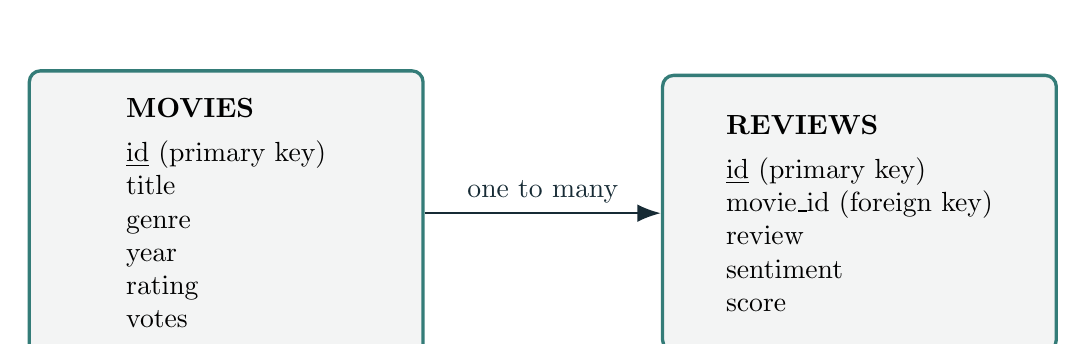
\begin{tikzpicture}[
  entity/.style={draw=teal, very thick, rounded corners, fill=lightgray,
                 minimum width=5.0cm, minimum height=3.5cm, align=left,
                 inner sep=10pt},
  relation/.style={-{Latex[length=3mm]}, thick, draw=ink},
  node distance=3.0cm
]
  \node[entity] (movie) {\textbf{MOVIES}\\[4pt]
    \underline{id} (primary key)\\
    title\\ genre\\ year\\ rating\\ votes};
  \node[entity, right=of movie] (review) {\textbf{REVIEWS}\\[4pt]
    \underline{id} (primary key)\\
    movie\_id (foreign key)\\
    review\\ sentiment\\ score};
  \draw[relation] (movie.east) -- node[above, text=ink] {one to many} (review.west);
\end{tikzpicture}
\end{center}

\begin{table}[h]
\centering
\caption{Logical database schema}
\begin{tabularx}{\textwidth}{>{\raggedright\arraybackslash}p{2.5cm} X X}
\toprule
\textbf{Table} & \textbf{Fields} & \textbf{Purpose} \\
\midrule
\texttt{movies} & \texttt{id}, \texttt{title}, \texttt{genre}, \texttt{year}, \texttt{rating}, \texttt{votes} & Stores movie identity and rating metadata. \\
\texttt{reviews} & \texttt{id}, \texttt{movie\_id}, \texttt{review}, \texttt{sentiment}, \texttt{score} & Stores review text and the computed sentiment result; \texttt{movie\_id} links each row to a movie. \\
\bottomrule
\end{tabularx}
\end{table}

\chapter{Implementation}
\textit{This section describes the methodology and approach; source code is not included, as requested by the report template.}

\begin{enumerate}
  \item \textbf{Data preparation:} The R preparation script downloads the pinned source files, combines the genre metadata, removes duplicate title/year pairs, and matches movies to their review files. It selects 200 movies using a fixed random seed and samples up to 30 non-empty reviews for each selected movie.
  \item \textbf{Data structures and import:} The records are represented as R data frames. The application reads \texttt{movies.csv} and \texttt{reviews.csv}, then loads them into the local \texttt{movies} and \texttt{reviews} SQLite tables.
  \item \textbf{Sentiment function:} Each review is converted to lowercase and split into words. A fixed positive and negative word list is used to count polarity matches. If one of a set of negators appears in the three preceding tokens, the matched word's polarity is reversed. The normalized result is mapped to a score from 0 to 1: scores at or above 0.575 are Positive, scores at or below 0.425 are Critical, and scores between these thresholds are Mixed. Text with no matching words receives a neutral score of 0.5 and the Mixed label.
  \item \textbf{Interactive search:} A Shiny event handler reads the search field and uses a case-insensitive substring match against movie titles. Matching results are displayed with movie metadata and sampled reviews.
  \item \textbf{Analysis and plots:} \texttt{dplyr} groups and summarizes the sample. \texttt{ggplot2} displays rating comparisons, year trends, and sentiment distributions. Shiny outputs update in response to the selected tab, filters, or movie search.
  \item \textbf{Persistence:} DBI and RSQLite connect the app to a local SQLite file. Movie IDs link review records to the correct movie. On later starts, newly prepared title/year records can be added while existing database rows are kept.
\end{enumerate}

\chapter{Output}
The application presents a dashboard with movie search, overview, genre study, audience voice, and movie explorer views. The following example uses a movie that is present in the local sample.

\begin{lstlisting}
SCREEN / SENSE - Example movie result
Title: Inception
Genre: Action
Year: 2010
IMDb rating: 8.8 / 10
IMDb votes: 1,981,675
Sampled reviews: 30

Lexicon sentiment in the 30 sampled reviews:
Positive: 23
Mixed:     6
Critical:  1
\end{lstlisting}

The sample-level summary is 200 movies, 6,000 reviews, 13 primary genres, and an average IMDb rating of approximately 7.89 out of 10. Across the sampled reviews, the lexicon labels 75.7\% Positive, 16.6\% Mixed, and 7.7\% Critical. These percentages describe the current sample only.

\chapter{Results and Discussion}
The application successfully organizes the local movie records and makes the sample searchable. It produces summaries at the movie and genre levels and visualizes rating and sentiment patterns over the available release years. The database relationship keeps each review associated with its movie, while the fixed sample seed makes the preparation results repeatable.

The sentiment method is easy to explain and useful for demonstrating text processing, functions, and conditional classification in R. However, it is a simple heuristic rather than a trained language model. It can miss synonyms, misunderstand context or sarcasm, and perform poorly on non-English text. Negation handling is limited to a short preceding window. IMDb ratings are source-provided values, while sentiment labels are computed by this project; they should not be treated as equivalent measures.

\chapter{Conclusion and Future Work}
SCREEN / SENSE demonstrates how R can be used to import, transform, summarize, visualize, and interact with a real dataset. It combines data frames, user-defined functions, loops, conditions, Shiny reactivity, \texttt{dplyr}, \texttt{ggplot2}, and SQLite persistence in one application. The resulting dashboard supports exploratory analysis of movie ratings and sampled audience reviews.

\section*{Future Work}
\begin{itemize}
  \item Expand the catalogue with a current, documented source and preserve data provenance.
  \item Add more representative and multilingual review samples where licensing permits.
  \item Compare the lexicon baseline with a validated sentiment model and report evaluation metrics.
  \item Add filters for year, genre, and rating and allow users to export summaries.
  \item Improve handling of negation, intensifiers, context, and review language.
\end{itemize}

\chapter{References}
\begin{enumerate}
  \item MansaT. \textit{IMDb Movie Dataset}. Hugging Face Datasets. Available at: \url{https://huggingface.co/datasets/MansaT/Movie-Dataset}. Accessed 19 November 2026.
  \item Posit. \textit{Shiny: Build Interactive Web Apps with R}. Available at: \url{https://shiny.posit.co/}.
  \item Wickham, H., François, R., Henry, L., Müller, K., and Vaughan, D. \textit{dplyr: A Grammar of Data Manipulation}. R package documentation. Available at: \url{https://dplyr.tidyverse.org/}.
  \item Wickham, H. \textit{ggplot2: Elegant Graphics for Data Analysis}. Springer. Package documentation: \url{https://ggplot2.tidyverse.org/}.
  \item R Core Team. \textit{R: A Language and Environment for Statistical Computing}. R Foundation for Statistical Computing. Available at: \url{https://www.r-project.org/}.
  \item RSQLite and DBI package documentation. Available at: \url{https://rsqlite.r-dbi.org/} and \url{https://dbi.r-dbi.org/}.
\end{enumerate}

\end{document}
